% mn2eguide.tex
% v2.1 released 03/05/2002
%
% Adapted from mnguide.tex
% v1.3 released 14th September 1995
% v1.2 released 5th September 1994 (M. Reed)
% v1.1 released 18th July 1994
% v1.0 released 28th January 1994


% The journal style files and macros, with guides on their use, are
% available by anonymous FTP on the Internet from the Comprehensive
% TeX Archive Network (CTAN) sites ftp.tex.ac.uk and ftp.dante.de.
% The files are in the directories
% /tex-archive/macros/plain/contrib/mnras and
% /tex-archive/macros/latex209/contrib/mnras for the TeX and LaTeX
% files respectively.



\documentclass[useAMS,usenatbib]{mnras}

\usepackage{rotating}
\usepackage{lscape}
\usepackage{graphicx}
\usepackage{amssymb}
\usepackage{amsmath}
\usepackage{epstopdf}
\usepackage{color}
\usepackage{soul}
\usepackage{multirow}
\usepackage{longtable}
\usepackage{textcomp}
\usepackage[caption=false]{subfig}
\usepackage{float}
\usepackage{appendix}
\usepackage{listings}

\def\mnras{MNRAS}
 \def\apj{Astrophys. J.}
 \def\aap{Astron. Astrophys.}
 \def\apjs{Astrophys. J., Suppl. Ser.}



%--------------------------------------------------------
\bibliographystyle{mn2eNicola}

\usepackage{hyperref}

\title[HELP:XID+]
  {HELP: XID+, The Probabilistic De-blender for Herschel SPIRE maps}\author[P.D. Hurley et al.]{P.D.~Hurley,$^1$\thanks{Email: p.d.hurley@sussex.ac.uk} S.~Oliver,$^1$ and other HELP team members\\
$^1$Astronomy Centre, Department of Physics and Astronomy, University of Sussex, Falmer, Brighton BN1 9QH, UK\\}

\date{Released 2002 Xxxxx XX}

\pagerange{\pageref{firstpage}--\pageref{lastpage}} \pubyear{2002}

\def\LaTeX{L\kern-.36em\raise.3ex\hbox{a}\kern-.15em
    T\kern-.1667em\lower.7ex\hbox{E}\kern-.125emX}

\newtheorem{theorem}{Theorem}[section]
\graphicspath{}
\begin{document}

\label{firstpage}
\maketitle

\begin{abstract}
As part of the Herschel Extragalactic Legacy Project (HELP), we have developed a new prior based source extraction tool, \emph{XID+}, to carry out prior source extraction on the Herschel SPIRE maps covered by HELP. \emph{XID+} is developed using a probabilistic Bayesian framework which provides a natural framework in which to introduce prior information, and uses the Bayesian inference tool \emph{Stan} to obtain the full posterior probability distribution on flux estimates. In this paper, we discuss the details of \emph{XID+} and demonstrate the basic capabilities and performance by running it on simulated SPIRE maps resembling the COSMOS field, and comparing to the current prior based source extraction tool \emph{DESPHOT}. We show that not only does \emph{XID+} perform better on metrics such as flux accuracy and flux density error, we illustrate how obtaining the posterior probability distribution can help overcome some of the inherent issues associated with maximum likelihood based source extraction routines. We also discuss how additional work within HELP will be utilised by \emph{XID+}.
Software available at \url{https://github.com/pdh21/XID_plus/}.
\end{abstract}


\begin{keywords}
galaxies: statistics -- infrared: galaxies
\end{keywords}
%
%
\section{Introduction}
%Infrared astronomy
Ever since the discovery of the far-infrared background with the \emph{Cosmic Background Explorer} (COBE) \citep{Puget:1996}, surveys have aimed to observe and detect the sources responsible for the emission. Most of those sources are galaxies, with the far-infrared emission coming from dust. 

While ground based observatories such as SCUBA \citep{SCUBA}, and more recently SCUBA-2 \citep{SCUBA2} and ALMA can make use of gaps in the infrared window to observe at the Rayleigh-Jeans tail of the far-infrared background, only space based facilities can observe at the peak. The first infrared space telescope, the InfraRed Astronomical Satellite (IRAS; \cite{Neugebauer:1984}), observed the whole sky in four bands centred at 12, 25, 60 and 100 $\mu m$ and revealed new populations of galaxies which were optically faint but luminous in the infrared \citep{Soifer:1984}.

While the Infrared Space Observatory (ISO; \cite{Kessler:1996}) and the Spitzer Space Telescope \citep{Werner:2004} have provided deep near and mid-infrared photometry over small fields, other smaller space based facilities such as AKARI \citep{Murakami:2007} and the Wide-field Infrared Survey Explorer (WISE, \cite{Wright:2010}) have surveyed the entire sky at mid to far-infrared and near to mid infrared wavelengths respectively. The most recent advancement in infrared astronomy has been made with the ESA Herschel Space Observatory \citep{Pilbratt:2010}. Photometry from the Photoconductor Array Camera and Spectrometer \citep[PACS][]{Poglitsch:2010} and Spectral and Photometric Imaging Receiver \citep[SPIRE][]{Griffin:2010} instruments have given us an unprecedented view of the far-infrared Universe by providing observations that measure across the peak of the far-infrared background and at greater sensitivity and resolution than has been achieved at these wavelengths.

With surveys such as the Herschel Multi-Tiered Extragalactic Survey (HerMES; \cite{Oliver:2012}) and the Herschel ATLAS survey (H-ATLAS; \cite{Eales:2010}), over 1000 square degrees of the sky has been observed by the SPIRE instrument. However, the limited resolution of the SPIRE photometer and high source density at the SPIRE wavelengths introduces two problems when trying to combine SPIRE data with existing multi wavelength data. 

The large beam size and low signal to noise of the SPIRE data results in large positional uncertainties for SPIRE detected sources. This makes matching to catalogues at other wavelengths difficult, as there may be more than one potential counterpart within the positional errors of the SPIRE detected source.

The second problem is that of source confusion. At the wavelengths observed by SPIRE, there is a high source density. This can often result in multiple sources being located within the SPIRE beam and, in extreme cases, lead to multiple astronomical sources being associated with one SPIRE detected source. 

To obtain accurate photometry from the SPIRE maps, overcoming the source confusion problem is essential. One way to solve the problem is to use prior information to accurately separate out the flux in the SPIRE maps to the underlying astronomical objects. For example, if we know the precise location of a galaxy (e.g. from an optical image where resolution is better), we expect a galaxy to be found in the SPIRE maps at the same location.

Several techniques have been developed that utilise the positions of sources detected at other wavelengths, usually 24 $\mathrm{\mu m}$ and 1.4 GHz, to disentangle the various contributions from discrete sources to the SPIRE flux in a given beam element \citep[e.g.][]{Roseboom:2010, Roseboom:2011, Chapin:2011}. This process is made possible by the high correspondence between the 24-$\mathrm{\mu m}$ and 1.4-GHz populations and those observed at far-IR wavelengths; $>$80 per cent of the cosmic IR background at SPIRE wavelengths can be accounted for by 24-$\mathrm{\mu m}$ sources with S24 $>$ 25 $\mathrm{\mu Jy}$ \citep[e.g.]{Marsden:2009, Pascale:2009, Elbaz:2010}, while the strong correlation between the far-IR and radio luminosity is known to hold across a wide range in redshift and luminosity \citep[e.g.][]{Ivison:2010}. Up to the present day, most of these techniques have used a maximum likelihood optimisation approach. However, \cite{Safarzadeh:2015} have recently used an MCMC based approach to fit PACS simulated maps, using prior information on position and flux.
 
The 24 $\mathrm{\mu m}$ XID algorithm, used by HerMES \citep{Roseboom:2010, Roseboom:2011} used a source list taken from the 24-$\mathrm{\mu m}$ source catalogue to introduce positional priors for sources in the 250, 350 and 500 $\mathrm{\mu m}$ maps. The same method was also used to produce HerMES DR2 source catalogues, with 250 $\mathrm{\mu m}$ sources as priors \citep[DESPHOT]{Wang:2014}. 

As part of the \emph{Herschel Extragalactic Legacy Project} (HELP), we have developed an alternative prior based approach for source extraction in confusion dominated maps. Our new method, \emph{XID+}, is built upon a Bayesian probabilistic framework which provides a natural framework in which to introduce additional prior information. By using the Bayesian inference tool, \citep[\emph{Stan},][]{stan-software:2015,pystan-software:2015} to sample full posterior distribution, we are also able to provide more accurate flux density error estimates, whilst avoiding some of the issues associated with the maximum likelihood and L1-constrained fitting approach used by \emph{DESPHOT}. In this paper, we demonstrate that \emph{XID+} outperforms \emph{DESPHOT} when using just positional information. In Section \ref{sec:XID+} we discuss the algorithm, show how the software performs on simulated SPIRE maps in section \ref{sec:sims} and discuss how \emph{XID+} can make use of flux prior information, delivered by the HELP project (Hurley et al. in prep) in section \ref{sec:conc}.
 
\section{XID+ Algorithm}\label{sec:XID+}
The basic goal of XID+ is to use the SPIRE maps to infer the likely SPIRE flux of sources we already know about. Bayesian inference is well suited to these requirements. It allows the use of prior information and provides a posterior distribution of the parameter(s) after taking into account the observed data.  

As discussed previously, we also want to provide a framework to do science directly with the maps rather than adding the additional step of first creating catalogues, which in essence is a form of data compression.

We therefore adopt a Bayesian probabilistic modelling approach for our XID+ algorithm. It aims to:
\begin{itemize}
\item map out the posterior rather than the traditional maximum likelihood point estimate, thereby providing a precise measure of uncertainty. 
\item Extend the use of prior information beyond just using positional information about sources.
\end{itemize}

In the following section, we describe our \emph{XID+} algorithm. As this algorithm builds upon knowledge gained from the original XID (a.k.a \emph{DESPHOT}) algorithm used by HerMES \citep{Roseboom:2010, Roseboom:2011, Wang:2014}, we describe XID+ in the context of how it differs from \emph{DESPHOT}. 

%change ordering: 
%Basic equations--linear fit--DESPHOT(LASSO)--XID+ model (model and STAN)--
%segmentation:-- optimum--DESPHOT--XID+
%uncertianties and covariances: DESPHOT---XID+

\subsection{Basic Model}
Our data $\mathbf{d}$ are maps with $n_1 \times n_2 = M$ pixels. Our model assumes the map are formed from $n$ known point sources, with an unknown flux density $\mathbf{f}$. The point response function (PRF) tells us the contribution each source makes to each pixel in the map. As the SPIRE maps are mean subtracted, our model requires a global background level ($B$) and some unknown noise term ($\delta$). Our map can therefore be described as follows:

\begin{equation}
\hat{\mathbf{d}} = \sum\limits_{i=1}^M \mathbf{P_i}f_i + B + \delta
\label{eq:map}
\end{equation}
where $\mathbf{d}$ is the image, $\mathbf{P_i}$ is the PRF for source $i$, $f_i$ is the flux density for source $i$, $B$ is a global background estimate and $\delta$ is the noise term.

We can rewrite the above equation in the linear form:
\begin{equation}
\hat{\mathbf{d}} = \mathbf{Af} + \delta
\label{eq:map2}
\end{equation}
Where $A$ is the pointing matrix, an $M \times n+1$ matrix giving the contribution of sources and background to each pixel.

Our map $\mathbf{d}$ will have an associated, and measurable, variance and possibly covariance between the pixels, which we define here as $\mathbf{N_d} = \langle\delta\delta^T\rangle$. We define the likelihood as the Gaussian probability function for the data given the flux densities
\begin{equation}
L(\mathbf{f}) = p(\mathbf{d}|\hat{\mathbf{f}}) \propto |\mathbf{N_d}|^{-1/2} \exp\big\{ -\frac{1}{2}(\mathbf{d}-\hat{\mathbf{d}})^T\mathbf{N_d}^{-1}(\mathbf{d}-\hat{\mathbf{d}})\big\}\label{eq:likelihood}
\end{equation}
The maximum likelihood solution to this equation can be found by setting $\chi = (\mathbf{d}-\hat{\mathbf{d}})^T\mathbf{N_d}^{-1}(\mathbf{d}-\hat{\mathbf{d}})$, finding the minimum and rearranging such that:

\begin{equation}
\hat{\mathbf{f}}=(\mathbf{A^TN_d^{-1}A})^{-1}\mathbf{A^TN_d^{-1}A}\label{eq:mlm}
\end{equation}

Equation \ref{eq:mlm} can be solved directly, either by brute-force matrix inversion or via other linear methods. As discussed in \cite{Roseboom:2010, Roseboom:2011, Wang:2014}, linear approaches ignore prior knowledge that fluxes cannot have negative flux density.% which in very degenerative cases can result in any symmetric pairing of positive and negative flux providing a good fit.
 They are also incapable of discriminating between real and spurious sources, which can result in overfitting. To overcome these issues, \cite{Roseboom:2011} used the non-negative weighted LASSO algorithm \citep{Tibshirani:1996, Zou:2006, terBraak:2010}.

LASSO is a shrinkage and selection method for linear regression and works by treating sources either `inactive' and flux density set to zero, or `active'. It switches sources on one at a time, with the order determined by reduction in chi-squared gained by turning them on. The process continues until some tolerance is reached.

%In the first iteration,\emph{DESPHOT}uses LASSO on each segment, to estimate the source fluxes. It then estimates a value for the background (B) via
%\begin{equation}
%B = \mathbf{d} - \sum\limits_{i=1}^n \mathbf{P_i}f_i
%\end{equation} 
%
%The estimate from B is subtracted, and the LASSO fitting is rerun to get the final flux density estimates.

For \emph{XID+}, we want to map out the entire posterior, $p(\mathbf{f}|\mathbf{d})$, rather than find the maximum likelihood solution. This has the benefit that it gives us more accurate information about how certain we are about the predicted fluxes. The posterior can be defined as:
\begin{equation}
p(\mathbf{f}|\mathbf{d}) \propto p(\mathbf{d}|\mathbf{f}) \times p(\mathbf{f})
\end{equation}
where $p(\mathbf{d}|\mathbf{f})$ is our likelihood, defined in equation \ref{eq:likelihood} and $p(\mathbf{f})$ is our prior on the fluxes. 

In our probabilistic framework, we can illustrate our model for the map, defined in equation \ref{eq:map2} via a probabilistic graphical model (PGM). Figure \ref{fig:graph_mod_xid+} shows our PGM for our basic XID+ model, where boxes represent dimensions, open circles as random variables, dots as deterministic or (fixed) variables. For our simplest model, the sky co-ordinates of our sources are treated as deterministic (i.e. known). The PRF is also assumed to be known, and modelled as a Gaussian, with full-width half-maximum (FWHM) of 18.15, 25.15 and 36.3 arcsec for 250, 350 and 500 $\mathrm{\mu m}$ respectively. Both these deterministic variables are used to make the pointing matrix $A$ which gives the contribution each source makes to each pixel $j$ in the map. Each source has its own flux $f$ which is a random variable. By multiplying $f$, $A$ and adding our global estimate for the background $B$, we can make our model for the map, $M$. 
\begin{figure}
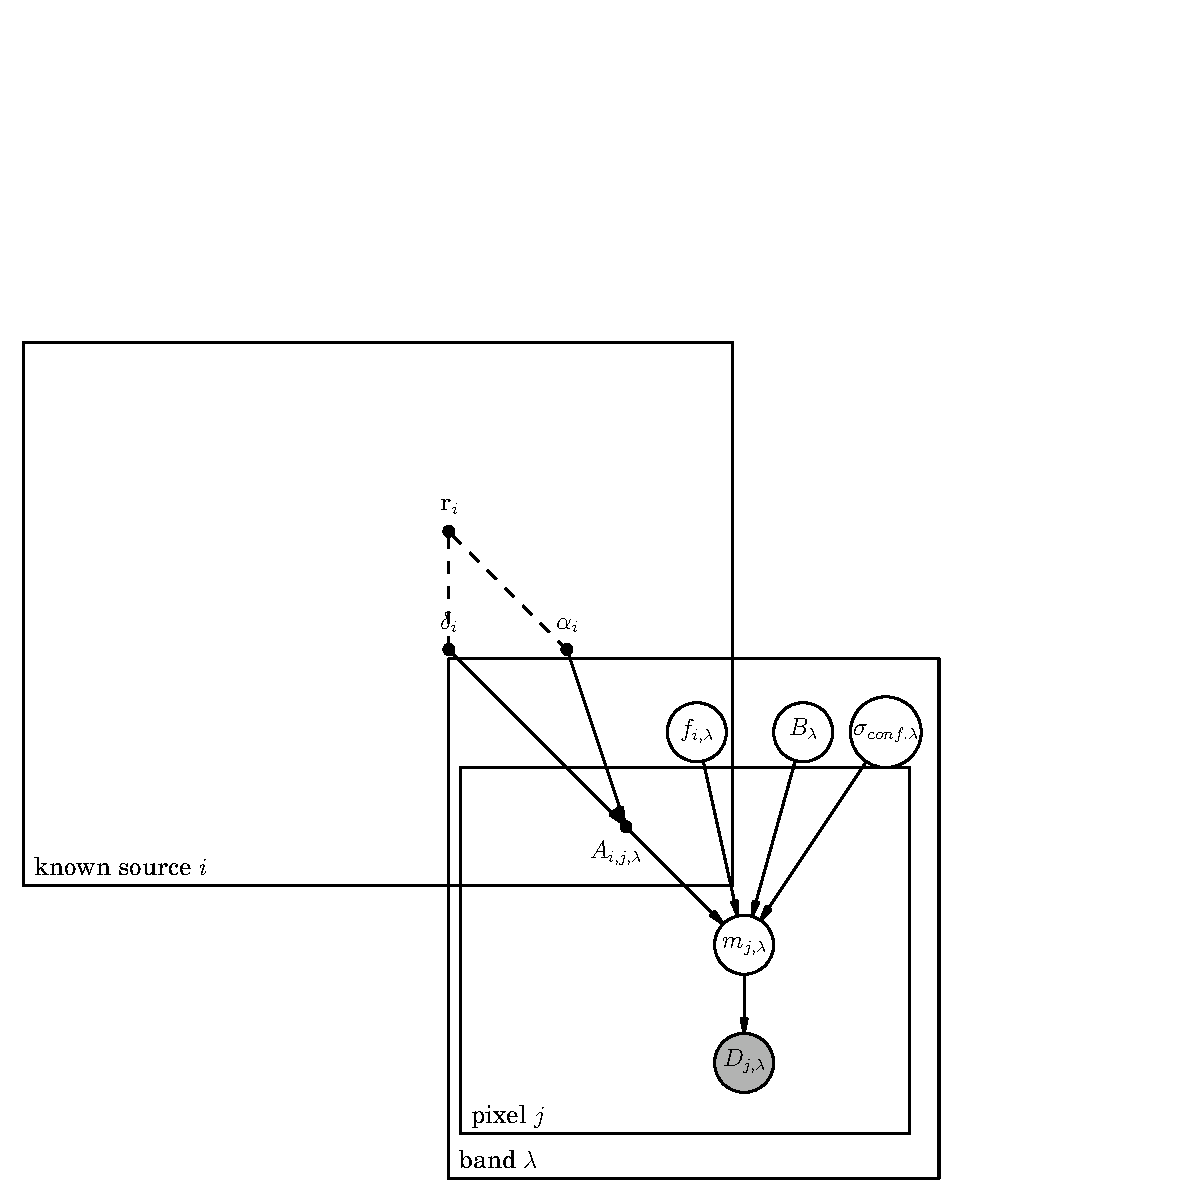
\includegraphics[width=8.5cm]{./graphical_model.pdf}
\caption{Our probabilistic model for XID+. Boxes represent dimensions, open circles as variables, dots as deterministic or (fixed) variables. Created with DAFT (\url{http://daft-pgm.org/})}\label{fig:graph_mod_xid+}
\end{figure}
 
\subsubsection{Stan}
Now we have our probabilistic model, we need a Bayesian inference tool capable of sampling from it to obtain the posterior. We use the Bayesian inference tool, \textit{Stan}, which is `a probabilistic programming language implementing full Bayesian statistical inference with MCMC sampling'. \textit{Stan} uses the adaptive Hamiltonian Monte Carlo (HMC) No-U-Turn Sampler (NUTS) of \cite{Hoffman:2013} to efficiently sample from the posterior. It does this by using the gradient information, allowing fast traversing of high dimensional and highly correlated joint posterior distributions. 

\textit{Stan} has its own modelling language, in which one constructs probabilistic models. Our model for \textit{Stan} can be found in Appendix A.
\subsubsection{Estimating Convergence}\label{sec:conv}
As with all MCMC routines, one needs to run enough chains and run them long enough to be confident the global minimum has been found and that it has been thoroughly sampled. 

As default, we run four separate chains from different initial positions. We also discard the first half of the chain as `warm up' to ensure the chains have converged to the posterior distribution. We then assess the convergence of each parameter by comparing the variation between and within chains using the diagnostics described in \cite{BDA3} which can be summarised as follows: Each chain is split in two and the between ($B$) and within chain ($W$) variance is calculated. $B$ and $W$ are then used to calculate the marginal posterior variance. This in turn can be used to estimate the potential scale reduction $\hat{R}$, which reduces to 1 as the number of iterations tends to infinity. An $\hat{R}$ value $> 1.2$ suggests chains require more samples. We provide $\hat{R}$ for each parameter.

Due to the nature of MCMC, samples from MCMC routines are correlated. Inference from correlated samples is less precise than from the same number of independent draws. In order to check there are enough independent draws we estimate the effective number of samples $\hat{n_{eff}}$, defined in \cite{BDA3}. We require $\hat{n_{eff}}$ to be 5 times the number of chains and provide the estimate for each parameter.

\subsection{Map segmentation}
The survey fields in HELP vary in size from 0.3 to 290 square degrees. Ideally, source photometry and background estimation would be done on the full image. In practice this will be computationally infeasible.\emph{DESPHOT} segmented the map by locating islands of high SNR pixels enclosed by low SNR pixels.

The most optimum and transparent way of segmenting the map would use distinct tiles but fitting for sources within and beyond the tiling region. Using the fact that, conditional on the fluxes, the data from each tile is independent, the posterior from the different tiles can be combined to give an overall posterior for the whole map using the following formula:

\begin{equation}
P(\mathbf{F}|D_1,..D_n,D_A)=a\frac{\prod_{i=1}^n P(\mathbf{F}|D_n,D_A)}{P(\mathbf{F}|D_A)^{n-1}}
\end{equation}

where $n$ is number of tiles and $P(\mathbf{F}|D_A)$ is our prior on the flux, given some ancillary data. As the number of dimensions is highly dimensional, the only feasible way of multiplying highly dimensional probability distribution functions is to model them as multivariate Gaussians. We investigated fitting the fluxes in both normal and log space, however in neither case was the multivariate Gaussian approximation appropriate.

We have settled on a tiling scheme that has tiles that overlap in the map. This makes sure sources that lie near the edge of a tile, will be nearer the centre of the adjacent tile. As before, for each tile, we fit to sources both in and beyond. For our final posterior, for each source, we take the posterior form the tile that is optimum, i.e. the tile in which the source lies closest to the centre.

\subsection{Uncertainties and Covariances}
\emph{DESPHOT} provides an estimate of the covariance matrix associated with the fluxes ($\mathbf{N_f}$) from $(\mathbf{A^TN_d^{-1}A})^{-1}$. Due to the Cramer-Rao inequality, this estimate is a lower limit. It also assumes the \emph{DESPHOT} algorithm is linear, which is not strictly true having introduced LASSO and non-negative priors. As a result, the uncertainties are unreliable. For \emph{XID+}, we have the full posterior, allowing the true variance to be properly characterised. This not only gives us a better estimate for marginalised uncertainty for each source, but it also provides the covariance information between sources (as seen in Figure \ref{fig:corr}). 
%
%An estimate of the remaining residual confusion noise is is calculated by taking the standard deviation of the residual map pixels $\sigma{res}$ and removing the average instrumental noise in these pixels in quadrature, $\sigma^2_{conf} = \sigma^2_{res} - \sigma^2_{pix}$, where $\sigma_{pix}$ is calculated directly from the exposure time per pixel. The total noise $\sigma_{tot}$ for a point source is then calculated from both the instrumental noise (and confusion noise from the known sources), $\sigma_{i} = \sqrt{\mathrm{diag}((\mathbf{A^TN^{-1}_dA)^{-1})}}$, and confusion noise from the unknown sources in the residual map $\sigma_{conf}$ via $\sigma^2_{tot} = \sigma^2_{i} + \sigma^2_{conf}$. 

%Details on what we get out of fit. e.g. marginalised estimate of fluxes, covariance information between sources

\begin{figure*}
\centering 
\subfloat{\includegraphics[width=5.5cm,page={4}]{metrics_XIDp.pdf}}
\subfloat{\includegraphics[width=5.5cm,page={5}]{metrics_XIDp.pdf}}
\subfloat{\includegraphics[width=5.5cm,page={6}]{metrics_XIDp.pdf}}\\[-2ex]
\subfloat{\includegraphics[width=5.5cm,page={4}]{metrics_DESPHOT.pdf}}
\subfloat{\includegraphics[width=5.5cm,page={5}]{metrics_DESPHOT.pdf}}
\subfloat{\includegraphics[width=5.5cm,page={6}]{metrics_DESPHOT.pdf}}
\caption{Inverse precision, or IQR of \emph{XID+} (top) and \emph{DESPHOT} (bottom) as a function of true flux, for the 250 (blue), 350 (green) and 500 (red) $\mathrm{\mu m}$ SPIRE bands. Black solid and dashed lines shows median and standard deviation respectively. Density of objects is illustrated via underlying colour. }\label{fig:precision}
\end{figure*}

\begin{figure*}
\centering 
\subfloat{\includegraphics[width=5.5cm,page={7}]{metrics_XIDp.pdf}}
\subfloat{\includegraphics[width=5.5cm,page={8}]{metrics_XIDp.pdf}}
\subfloat{\includegraphics[width=5.5cm,page={9}]{metrics_XIDp.pdf}}\\[-2ex]
\subfloat{\includegraphics[width=5.5cm,page={7}]{metrics_DESPHOT.pdf}}
\subfloat{\includegraphics[width=5.5cm,page={8}]{metrics_DESPHOT.pdf}}
\subfloat{\includegraphics[width=5.5cm,page={9}]{metrics_DESPHOT.pdf}}
\caption{Accuracy of \emph{XID+} (top) and \emph{DESPHOT} (bottom) as a function of true flux, for the 250 (blue), 350 (green) and 500 (red) $\mathrm{\mu m}$ SPIRE bands. Black solid and dashed lines shows median and standard deviation respectively. Density of objects is illustrated via underlying colour.}\label{fig:accuracy}
\end{figure*}

\begin{figure*}
\centering 
\subfloat{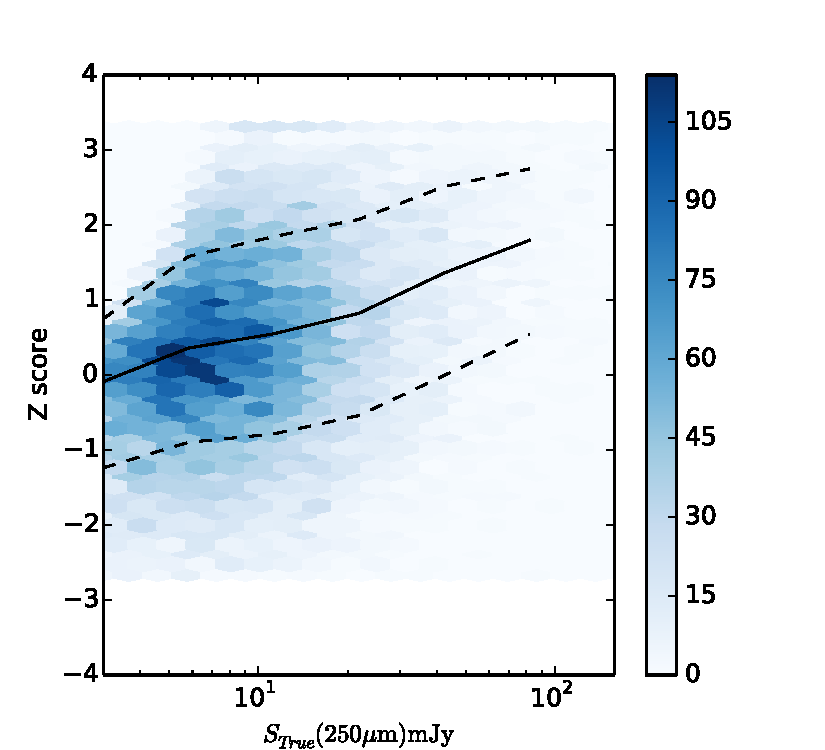
\includegraphics[width=5.5cm,page={1}]{metrics_XIDp.pdf}}
\subfloat{\includegraphics[width=5.5cm,page={2}]{metrics_XIDp.pdf}}
\subfloat{\includegraphics[width=5.5cm,page={3}]{metrics_XIDp.pdf}}\\[-2ex]
\subfloat{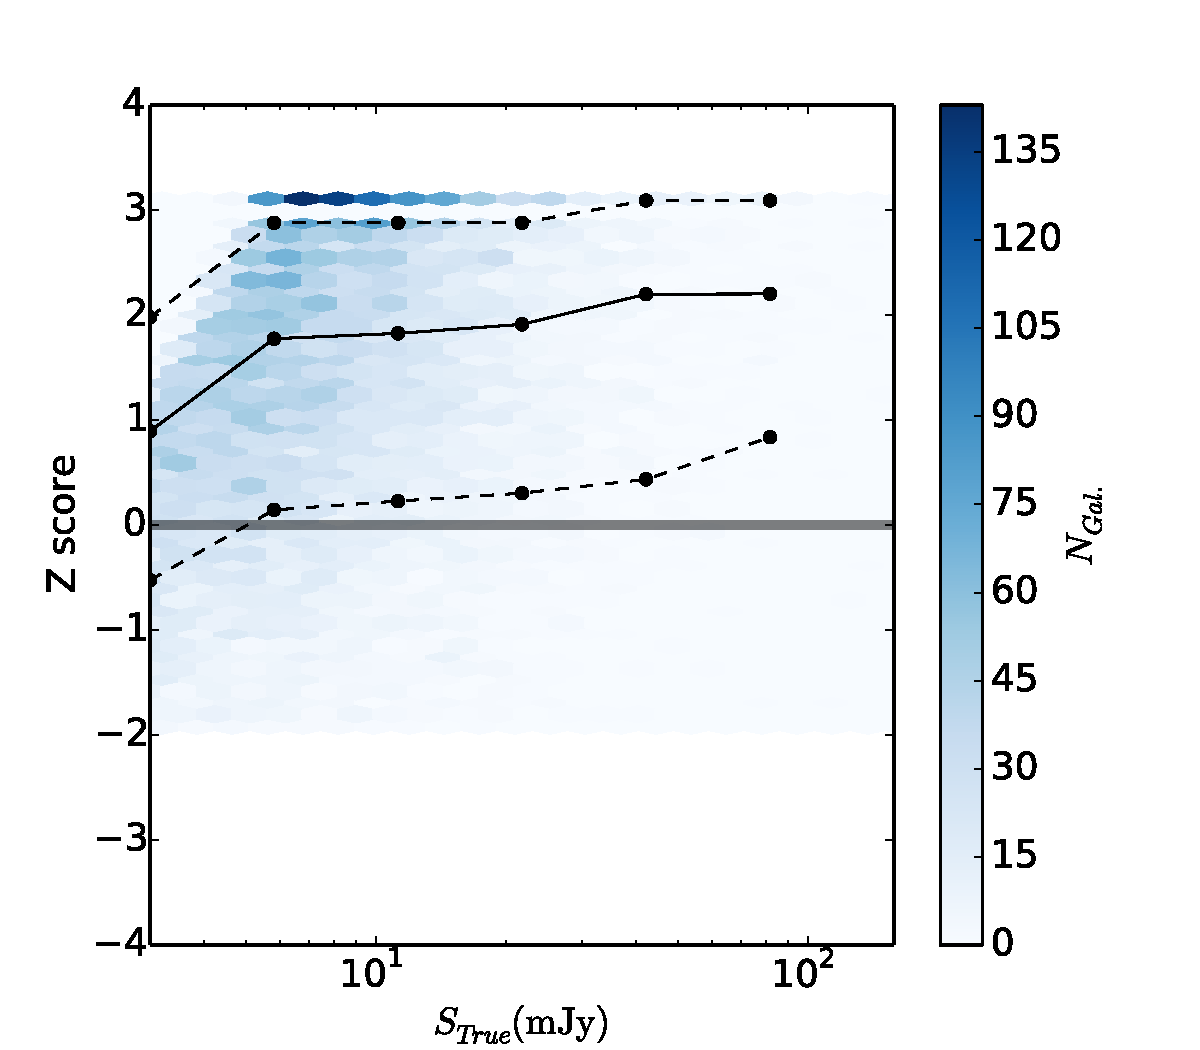
\includegraphics[width=5.5cm,page={1}]{metrics_DESPHOT.pdf}}
\subfloat{\includegraphics[width=5.5cm,page={2}]{metrics_DESPHOT.pdf}}
\subfloat{\includegraphics[width=5.5cm,page={3}]{metrics_DESPHOT.pdf}}
\caption{Z score, or flux density error for \emph{XID+} (top) and \emph{DESPHOT} (bottom) as a function of true flux, for the 250 (blue), 350 (green) and 500 (red) $\mathrm{\mu m}$ SPIRE bands. Black solid and dashed lines shows median and standard deviation respectively. Density of objects is illustrated via underlying colour.}\label{fig:zscore}
\end{figure*}

\section{Simulations}\label{sec:sims}
In order to test and quantify XID+, we use simulated SPIRE maps of the COSMOS field, a good example of a deep map i.e. where $\sigma_{conf.} \gg \sigma_{inst.}$. In order to get realistic clustering, we use the mock catalogues from the latest version of the Durham semi-analytic model, \emph{GALFORM}. (Lacey et al. in prep., also described in \cite{Cowley:2014}). The model is designed to populate Millennium-class, dark matter only, N-body simulations with a WMAP7 cosmology and minimum halo mass of $1.9 \times 10^{10} h^{-1} M_{\odot}$. The dust model is motivated by the radiative transfer code GRASIL \citep{Silva:1998} and can accurately reproduce the predictions for rest-frame wavelengths $\lambda_{rest} > 70 \mathrm{\mu m}$.

A mock 100 $\mathrm{\mu m}$ input catalogue, similar to that expected from a PACS catalogue, is generated by taking the mock catalogue and making a cut at a flux limit of 50 $\mathrm{mJy}$. We use this as our prior input catalogue for both \emph{XID+} and \emph{DESPHOT}. In order to compare performance, we look at three measures: precision, flux accuracy, and flux error density. For \emph{XID+}, we only consider sources whose output median flux is above $1\mathrm{mJy}$. Likewise, with \emph{DESPHOT}, we only consider sources which have a maximum likelihood flux of greater than $1\mathrm{mJy}$. 

\subsection{Flux Precision}
Precision is a measure of how well the flux is believed to be constrained. For our posterior sample, this relates to how spread out the sample is and so we use the interquartile range (IQR) as our measure of precision. Figure \ref{fig:precision} shows the 50th,84th and 16th percentile (i.e. median and median $\pm \sigma$) for 7 bins in true flux. IQR is normalised and as a function of input flux for both \emph{XID+} and \emph{DESPHOT}. As one would expect, $\mathrm{IQR}/S_{True}$ decreases as a function of input flux, indicating a higher precision is achieved for the brighter sources. While $250$ and $350\mathrm{\mu m}$ outputs achieve a similar level of precision, the outputs for $500 \mathrm{\mu m}$ do not reach the same level of precision. In comparison to \emph{DESPHOT}, \emph{XID+} is marginally worse for all three bands, though as we show later, this is linked to a better estimate of uncertainty. 

\subsection{Flux Accuracy}
Flux accuracy is a measure of how far away the estimated flux is from the truth. We use the difference between our median flux estimate from our posterior and the true flux from the simulation, normalised by true flux, as our estimate of flux accuracy. Figure \ref{fig:accuracy} shows how flux accuracy changes as a function of input flux for all three bands. As before, we show the 50th,84th and 16th percentile for 7 bins in true flux. For 250 $\mathrm{\mu m}$, $\emph{XID+}$ reaches a zero level by $\approx 5 \mathrm{mJy}$, where as \emph{DESPHOT} underestimates the flux for all but the very brightest sources. For 350 $\mathrm{\mu m}$ and 500 $\mathrm{\mu m}$, a zero level is reached by $\approx10 \mathrm{mJy}$, where as \emph{DESPHOT} continues to underestimate for all but the very brightest sources.

\subsection{Flux Error density}
Flux error density measures how well accurate the estimated uncertainty is correct. Estimated flux values should be within one sigma of the true value 68.27\% of the time and within 2 sigma 95.45\% of the time. Figure \ref{fig:zscore} shows the flux error density (or Z score) as a function of input flux. For \emph{DESPHOT}, uncertainties are assumed to have a normal distribution, truncated at zero. With \emph{XID+}, we have the full posterior and no longer have to make an assumption on the shape of the uncertainty distribution. Instead, we calculate error density by taking the percentile at which the true flux value falls within the posterior, and convert the percentile to a corresponding sigma level.

For the 250 $\mathrm{\mu m}$ band, and sources under $\approx25\mathrm{\mu Jy}$, \emph{XID+} produces a Z score distribution which that matches that expected if uncertainties are correctly estimated (i.e. distribution is centred around zero, with width $\approx 1$). Above $25\mathrm{\mu Jy}$, the median Z score increases, indicating flux and uncertainty is being under estimated. In comparison, for all fluxes, the uncertainty distribution from \emph{DESPHOT} is above 1, and increases to a Z score of over 2 for the brighter sources. This indicates that the majority of sources in \emph{DESPHOT} lie over 1 $\sigma$ away from their true flux. The flux error densities for 350 $\mathrm{\mu m}$ and 500 $\mathrm{\mu m}$ show a similar behaviour, though not as severe.

\subsection{Convergence}
As described in Section \ref{sec:conv}, we provide $\hat{R}$ as an estimate of convergence and $\hat{n_{eff}}$ as a measure of independence within the sample. Figures \ref{fig:converg} show the histogram for $\hat{R}$ and $\hat{n_{eff}}$ for the three bands, with our thresholds for the statistics shown by dotted lines. In our fit to the simulated SPIRE maps, we use four chains, each with 1500 iterations (half of which are discarded as warm up). This leads to over 99.99\% of the sources having an $\hat{R}$ and $\hat{n_{eff}}$ within the threshold for all three bands, indicating our solution is well converged. In cases where convergence has not been reached, the number of iterations can be increased.
\begin{figure}
\subfloat{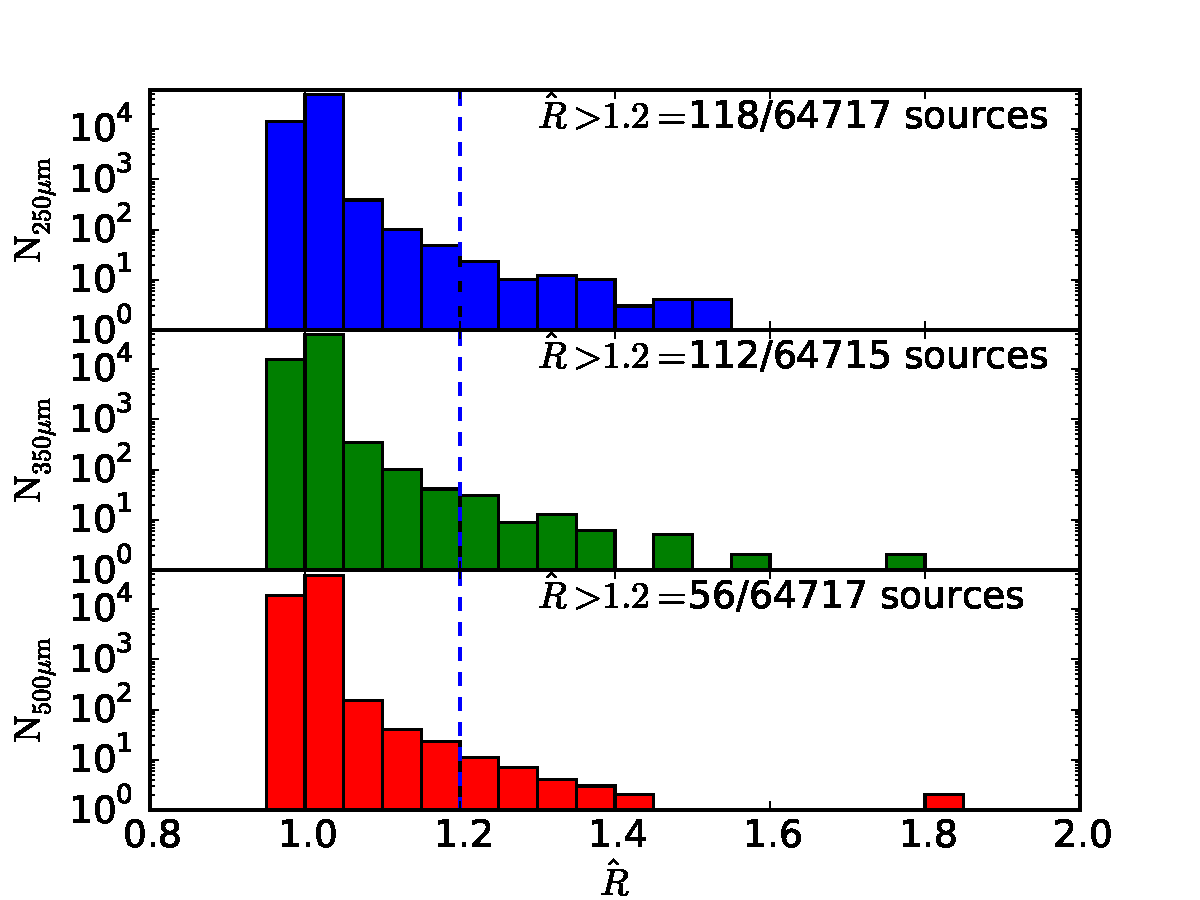
\includegraphics[width=6cm,page={1}]{convergence_test.pdf}}\\
\subfloat{\includegraphics[width=6cm,page={2}]{convergence_test.pdf}}
\caption{$\hat{R}$ and $\hat{n_{eff}}$}\label{fig:converg}
\end{figure}


\subsection{Remaining Noise}
The purpose of using prior based source extraction is to overcome the confusion noise in the SPIRE maps, which, as measured by \cite{Nguyen:2010} is 5.8, 6.3 and 6.8 $\mathrm{mJy}$ at 250, 350 and 500 $\mathrm{\mu m}$, respectively. By looking at the residual map (i.e. $\mathbf{d}-(\mathbf{Af}+B)$), we can estimate the remaining residual confusion noise in the maps.

We do this by measuring the standard deviation of the pixels in the residual map convolved with the PSF. This provides an estimate of the total noise remaining in the residual map ($\sigma_{tot.}$). In order to obtain an estimate of the confusion noise ($\sigma_{conf.}$), an estimate of the instrumental noise is made from the uncertainty map, and then removed in quadrature, such that $\sigma_{conf.}^2 = \sigma_{tot.}^2 - \sigma_{inst.}^2$. Table \ref{tab:remaining_noise} shows the total and confusion noise from the residual Lacey simulated maps, for both \emph{DESPHOT} and \emph{XID+}, and for all three SPIRE bands. For \emph{XID+}, we calculate a residual map (and remaining noise estimate) for each sample in the posterior, Table \ref{tab:remaining_noise} shows the median from the sample.

\begin{table}
\centering
\begin{tabular}{l|l|l|l|l|l|l|}
\cline{2-7}
                                       & \multicolumn{2}{l|}{$250\mathrm{\mu m}$} & \multicolumn{2}{l|}{$350\mathrm{\mu m}$} & \multicolumn{2}{l|}{$500\mathrm{\mu m}$} \\ \cline{2-7} 
                                       & $\sigma_{tot.}$     & $\sigma_{conf.}$    & $\sigma_{tot.}$    & $\sigma_{conf.}$    & $\sigma_{tot.}$   & $\sigma_{conf.}$    \\ \hline
\multicolumn{1}{|l|}{\emph{XID+}}    & 1.9                   & 1.3                   & 2.2                   &  1.9                   & 2.6                   &  1.9                   \\ \hline
\multicolumn{1}{|l|}{\emph{DESPHOT}} & 2.4                   & 1.9                 & 3.5                  &  3.3                 &  3.4                  &  2.9                   \\ \hline
\end{tabular}
\caption{Table showing the remaining total and confusion noise for the three SPIRE bands (in $\mathrm{mJy}$), from running \emph{XID+} and \emph{DESPHOT} on the Lacey simulated COSMOS maps.}
\label{tab:remaining_noise}
\end{table}
As demonstrated by the values in Table \ref{tab:remaining_noise}, \emph{XID+} reaches a confusion noise level substantially lower than the present in the maps. It is also lower than that achieved by \emph{DESPHOT}. This is could be due to the fact we fit the background simultaneously with the sources and/or the LASSO algorithm in\emph{DESPHOT} restricting the fit of close-by sources, hence increasing the flux variations in the residual map. 
 
\subsection{Correlated Sources}
For sources that are close together, the uncertainty on the flux estimates can be correlated. One of the advantages of obtaining the full posterior is we get a proper estimate of uncertainty and its correlation. This is particularly apparent when comparing flux estimates for with \emph{DESPHOT}, which, by using the LASSO algorithm forces one source to have all the flux and the other nearby source to zero. Figure \ref{fig:corr} shows an example of two correlated sources from our simulated map, and the estimate from both \emph{XID+} and \emph{DESPHOT}. The posterior provided by XID+, fully captures the correlated uncertainty, where as the `winner takes all' approach from \emph{DESPHOT} clearly fails to estimate the true flux for both sources.
 
\begin{figure} 
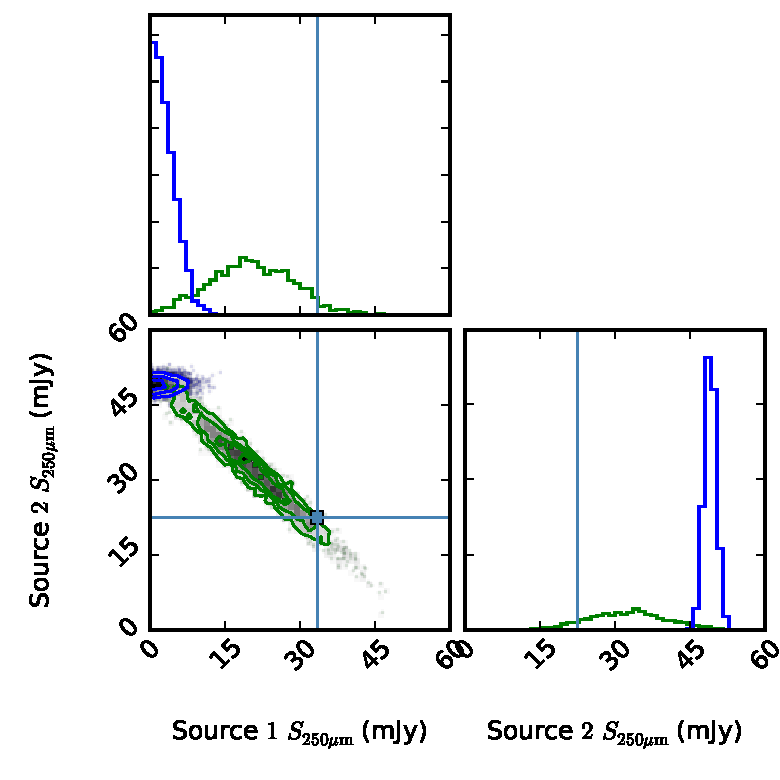
\includegraphics[width=6cm]{example_tri_DESHPOT_XIDp.pdf}
\caption{Posterior triangle plot of two correlated sources that are 2'' apart, with true fluxes indicated by the vertical and horizontal line. \emph{DESPHOT} (blue) assigns all the flux to one source, where as with \emph{XID+} we get the full uncertainty information from the posterior. Plot created with \protect\cite{triangle}.}\label{fig:corr}
\end{figure}
%\subsection{Real data}
% inject sources into map and recover

\section{Conclusions}\label{sec:conc}
In this paper we have introduced the prior based source detection software, \emph{XID+}. By using the Bayesian inference tool \emph{Stan}, we are able to fully sample the posterior probability, which in turn gives a better understanding of the uncertainty associated with the source flux. 

Having run XID+ on simulated maps, we have shown this is extremely advantageous for maps that are confusion limited, such as the \emph{Herschel} observations that are part of \emph{HerMES}. In comparison to the current maximum likelihood based software \emph{DESPHOT}, XID+ performs far better in all the three main metrics; flux accuracy, precision and uncertainty accuracy. 
 
By using a probabilistic approach, we have a framework where we can introduce prior information on the source fluxes in a transparent manner. For this basic version, we use a simple $\log_{10}$ uniform prior, with bounds at $10^{-2}$ and $10^{3}\mathrm{myJy}$. 

As can be seen in Figure \ref{fig:corr}, where sources are correlated, if we have prior knowledge on the flux of one of the sources, it can help us determine a more precise flux for the other.

As demonstrated by \cite{Safarzadeh:2015}, these priors could come from fitting spectral energy distribution models to multi-wavelength ancillary data. Another alternative is to use machine-learning algorithms to `learn' the expected flux from the statistical population. As part of HELP, the testing and benchmarking of suitable methods for deriving SPIRE flux priors will be presented in Hurley et al. (in prep). With \emph{XID+}, we now have the tool to be able to use that prior information in a clear and transparent way to obtain better SPIRE flux estimates, which is essential if we are to extract the wealth of information contained within in the Herschel maps.

\section*{Acknowledgements}%
%
%%
%
%
\bibliography{HELP_bib}
\appendix
\section*{Appendix A}\label{Stan_model}
\onecolumn
\lstinputlisting[language=C, linewidth=18cm]{../stan_models/XID+SPIRE.stan}
%
%
%
%
%
%%%%%%%%%%%%%%%%%%%%%%%%%%%%%%%%%%%%%
%
%% \bsp % ``This paper has been produced using the ...''
%
%\label{lastpage}

\end{document}
